\documentclass[UTF8,11pt,a4paper,fontset=none]{ctexart}
\setCJKmainfont[ItalicFont={Noto Serif CJK SC},SlantedFont={Noto Serif CJK SC}]{Noto Serif CJK SC}
\setCJKsansfont{Noto Sans CJK SC}
\setCJKmonofont{Noto Sans Mono CJK SC}
\usepackage{geometry,graphicx,booktabs,amsmath,fvextra,caption}
\usepackage[hidelinks]{hyperref}
\geometry{margin=2.5cm}
\DeclareCaptionFont{figuretext}{\zihao{5}}
\captionsetup[figure]{font=figuretext,justification=centering,singlelinecheck=false}
\setlength{\emergencystretch}{2em}
\ctexset{section={beforeskip=1.2ex,afterskip=0.8ex},subsection={beforeskip=1ex,afterskip=0.6ex}}
\setlength{\intextsep}{8pt}
\setlength{\textfloatsep}{8pt}
\newcommand{\promptbox}[1]{%
  \par\smallskip\noindent\begingroup
  \setlength{\fboxsep}{2mm}\setlength{\fboxrule}{0.4pt}%
  \fbox{\begin{minipage}{\dimexpr\linewidth-2\fboxsep-2\fboxrule\relax}
  \normalsize #1\end{minipage}}\endgroup\par\smallskip}
\begin{document}
\pagestyle{plain}
\begin{center}
{\LARGE\bfseries AI工具使用详情}\\[0.7em]
2026年9月13日
\end{center}

\section{工具及模型接口}
通过OpenCode接入DeepSeek V4.1 Flash API。

\section{具体使用目的}
\textbf{文章润色：}辅助调整论文的语言表达、段落衔接和术语使用，改善图文说明的清晰度与一致性并按照要求完成相应图的构建。

\textbf{代码调试：}辅助检查代码逻辑、定位运行异常与输入输出不一致问题，提出修改建议，并协助设计验证样例。对生成或修改的代码是否采纳则由人工核验结果决定。

\section{主要提示方式与使用过程说明}
以下以流程图生成和代码调试为例说明提示方式。提示文字为说明性整理，不作为逐字会话记录；代码片段仅用于演示局部判断逻辑。

\subsection{流程图生成示例}
\textbf{提示要求：}
\promptbox{
请根据圆柱形药材烘干模型，生成一张代码运行与核验流程图，依次展示“读取初态与边界、建立网格与模型、执行数值积分、检查全域含水率、整理与输出结果、人工核验后采纳”。采用黑色线条、简洁箭头和与论文一致的中文字体，合理安排节点，避免文字与连线重叠。
}

根据上述要求整理得到图\ref{fig:ai-flow}。人工审阅时检查流程顺序、节点含义和图文对应关系，再调整字体、间距及箭头位置。
\begin{figure}[!htbp]\centering
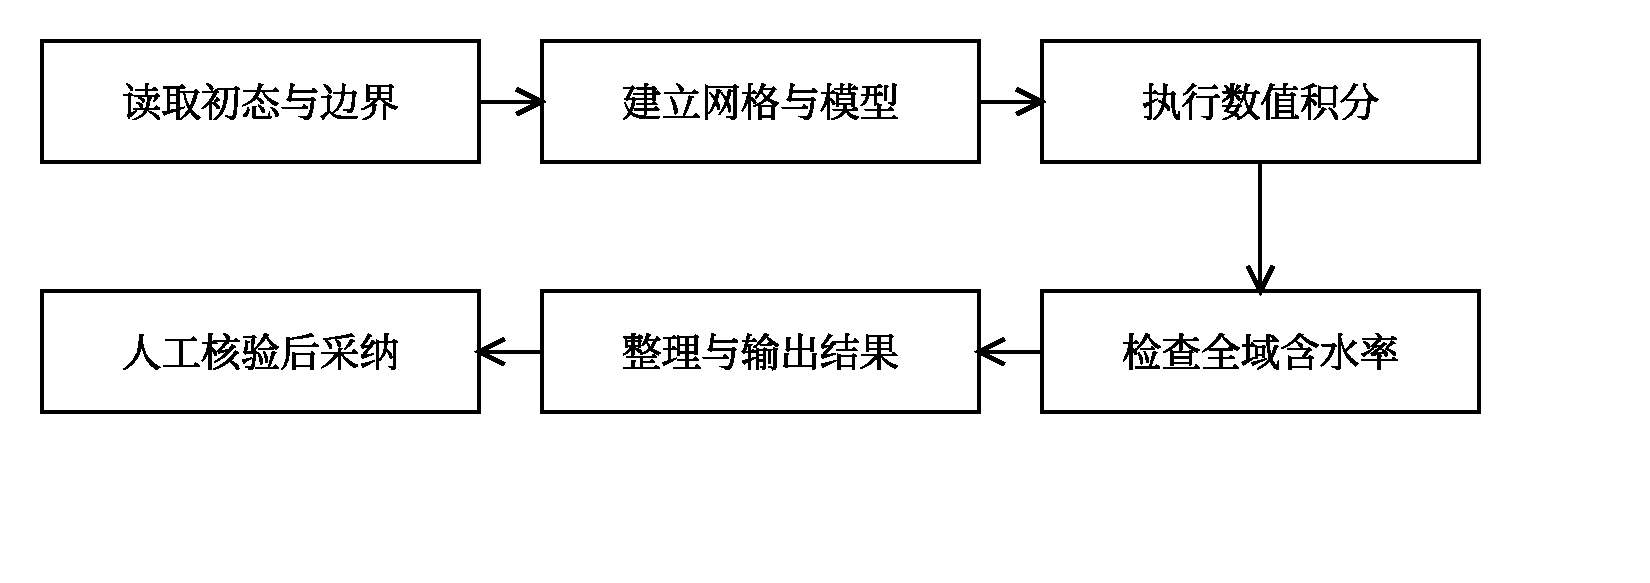
\includegraphics[width=\linewidth]{figures/ai_usage_flow.pdf}
\caption{代码运行与核验流程示例}\label{fig:ai-flow}
\end{figure}

\clearpage
\subsection{代码调试示例}
\textbf{待修正代码：}
\begin{Verbatim}[fontsize=\small,frame=single,framerule=0.4pt,framesep=2mm]
rounded = [round(c, 4) for c in state]
finished = max(rounded) < 0.15
\end{Verbatim}

\textbf{修改提示：}
\promptbox{
请检查以上含水率终点判定代码。当最大含水率为0.14996时，保留四位小数后变为0.1500，导致判断结果与原始数值不一致。请使用未舍入数值判断是否严格小于0.15，将四舍五入仅用于显示，并补充阈值以下、等于阈值和高于阈值的检查样例。
}

修改后的代码见图\ref{fig:corrected-code}。
\begin{figure}[htbp]\centering
\begin{Verbatim}[fontsize=\small,frame=single,framerule=0.4pt,framesep=2mm]
def drying_finished(values, threshold=0.15):
    values = tuple(values)
    if not values:
        raise ValueError("empty concentration data")
    return max(values) < threshold
state = [0.14996, 0.12000, 0.05270]
finished = drying_finished(state)
# Round for display only, after the decision.
display_values = [round(c, 4) for c in state]
\end{Verbatim}
\caption{终点判定示例的修改后代码}\label{fig:corrected-code}
\end{figure}

\textbf{示例运行检查：}保持其余位置的含水率低于阈值，分别令最大值为0.14996、0.15000和0.15004，修改后人工核验后判定依次为“达标、未达标、未达标”，符合严格小于0.15的要求。

\section{采纳情况}
最终采纳的AI生成或修改代码，均在经过人工完整核验，确认其能够正常运行并输出符合预期的结果后予以采用。未通过核验或输出结果不符合预期的代码则不予采纳。

文章润色建议同样经过人工审阅，以确保表述准确、逻辑连贯，且未改变原有模型、数据及结论。AI输出作为辅助材料使用，最终内容的取舍还是由人工决定。
\end{document}
